%!TEX root = ../../thesis.tex
\define{\chapterpath}{\allchapterspath/conclusion}
\define{\imgpath}{\chapterpath/img}

\chapter{Conclusion}
\label{chapter:conclusion}
\minitoc

In this thesis, we have developed a set of algorithmic solutions to deal with the problem of \emph{learning from unlabeled interaction frames}. We proposed several methods to exploit the assumption that users are coherent in their teaching behaviors, and to allow the learning agent to improve its performance by actively selecting its next actions.

In this chapter, we summarize our contributions and highlight the most important ideas and algorithm properties of this work. Finally, we explicit a number of possible directions for future research in this domain. We particularly highlight two important directions. The first is to study the property of our problem in a more theoretical way (e.g. convergence properties, effects of world properties). The second direction is the importance of testing this algorithm with a multitude of users in a variety of tasks, we particularly highlight the potential difference between intuitive and adaptive interfaces. As a final note, we highlight the challenge of learning new meanings and identifying new frames through practical interaction with humans.

%%%%%%%%%%%%%%%%%%%%%%%%%%%%%%%%%%%%%%%%%%%%%%
%%%%%%%%%%%%%%%%%%%%%%%%%%%%%%%%%%%%%%%%%%%%%%
%%%%%%%%%%%%%%%%%%%%%%%%%%%%%%%%%%%%%%%%%%%%%%
%%%%%%%%%%%%%%%%%%%%%%%%%%%%%%%%%%%%%%%%%%%%%%
%%%%%%%%%%%%%%%%%%%%%%%%%%%%%%%%%%%%%%%%%%%%%%
\section{Summary of contributions}

In this paper we have shown that, given a limited number of possible tasks, it is possible to solve sequential tasks using human feedback without defining a map between feedback signals and their meaning beforehand. The proposed algorithm optimizes a pseudo-likelihood function and performs active planing according to the the uncertainty in the task and meaning spaces. Indeed, taking into account this uncertainty is crucial to solve the task efficiently and to recover the actual meanings. This combination allows: 
\begin{inparaenum}[a)]
\item a human to start interacting with a system without calibration;
\item to automatically adapt calibration time to the user needs which can even outperform fixed calibration procedures; 
\item to adapt to the uncertainty of the information source from scratch.
\end{inparaenum}
We showed the applicability of the approach to brain-machine interfaces based on error potentials which could work out of the box without calibration, a long-desired property of this type of systems. 


%%%%%%%%%%%%%%%%%%%%%%%%%%%%%%%%%%%%%%%%%%%%%%
%%%%%%%%%%%%%%%%%%%%%%%%%%%%%%%%%%%%%%%%%%%%%%
%%%%%%%%%%%%%%%%%%%%%%%%%%%%%%%%%%%%%%%%%%%%%%
%%%%%%%%%%%%%%%%%%%%%%%%%%%%%%%%%%%%%%%%%%%%%%
%%%%%%%%%%%%%%%%%%%%%%%%%%%%%%%%%%%%%%%%%%%%%%
\section{Take home messages: ideas and algorithm properties}

\subsection{Two modes}

This subsection is meant to re-explain, from a slightly different perspective the ideas and structure behind the different steps of our algorithm. The readers that understand all the aspects of the algorithm can safely skip this subsection.

The algorithm is divided into a classification algorithm, estimating one classifier for each hypothesis based on past interaction, and a filtering algorithm that uses the predictions and properties of this classifier to update a belief over all tasks hypothesis.

The key point is that each hypothesis is considered as if it was the true one. We model the signal to meaning mapping of the user with respect to each task. We then simply test if each classifier can make accurate predictions. As the user is acting according to only one hypothesis, only that hypothesis will be able to predict correctly future interactions.

% Our assumptions is that the hypothesis which show more coherence between expected label and predicted label.

As we have detailed previously, once a task is correctly identified, we have access to the true intended labels of the user. Therefore we should be able to learn a second task faster. We now try to highlight the different processes acting during a full experiment of learning multiple tasks. We will refer to two phases: \begin{inparaenum}[a)] \item phase 1 is learning the first task from unlabeled instructions, and \item phase 2 is learning a second (or third, or \ldots) task knowing we already inferred a first task. \end{inparaenum} Our algorithm is the same for the two phases but different properties are more or less active during phase 1 or phase 2.

Phase 1 is the main contribution of this work. It enables a system to be instructed a new task using signals whose associated meanings are initially unknown. As stated before, our method generates interpretation hypothesis over the possible tasks, infers the hypothetic labels associated to the signals, computes a classifier for each hypothetic set of signal-label pairs, and assumes the one of better quality corresponds to the one the user has in mind. What really have an important impact during phase 1 is not the raw predictions of each classifier, but our measure of uncertainty on their predictions. Indeed, with very few data available, most classifiers are unable to predict correctly unseen data. Even the classifier associated to the correct task might be initially of bad quality, because of the noise in the teaching signals. Therefore all classifiers are considered as unreliable, and our Equation makes only small updates each step. It is only once one classifier stand apart as being more reliable than the others that differences between likelihoods will emerges.

% By doing so the system ends up knowing what is the task taught by the teacher and consequently what are the true labels associated to the teaching signals. Consequently, at the end of phase 1, the system knows a lot more about the mapping between human signals and their meaning.

Phase 2 is almost the contrary. After the first task is correctly identified, we have access to the true labels associated to each signals. One option may be to train a common classifier and consider the teaching as a known source of information. That way learning a second task should be a lot faster as the signal to meaning mapping is known. But this might not be the best option as phase 1 can be quite efficient to identify a first task. For example, as we will see in chapter~\ref{chapter:bci}, it is possible to identify a task in less than 100 iterations using brain signals, while a usual calibration procedure takes around 400 steps. If we stopped after the first task is identified, we could only use 100 signal-label pairs to train a classifier. This classifier is likely to be sub-optimal, making more classification errors. We will indeed observe that a classifier trained on 200 samples makes more errors than one trained on 400 samples.

Our algorithm improves over this approach. After phase 1, we only assign the true labels to all hypothesis. But we keep our hypothesis based approach, as in phase 1, which means we keep updating all the classifiers. Obviously, all classifiers will be very similar, and we maintain similar learning properties than when using a common classifier for each task, i.e. we discriminate the tasks faster. But the key point is that we continue using interpretation hypothesis, generating new signal-label pairs, potentially different for each task. And as wrong hypothesis will add wrong signal-label pairs to their classifiers, the quality of their classifier will also reduce, therefore reducing the sharpness, and quality, of their predictions; which we take into account in our updates. Obviously this effect will be quite small compared to phase 1 because an increasing number of signal-label pairs are shared between hypothesis. But it allows for a smooth transition between the two regimes of our algorithm. Indeed, the more task are identified, the more data are shared between classifiers, and the more signal-label pairs are needed to modify the properties of a classifier. We will see in later experiments with brain signals that the process used in phase 2 reduces the number of mistakes made by the system, especially when the number of teaching signals is still low.

% In the beginning phase 2, all the classifiers are the same, the difference between hypothesis will be on the match between classified signal and expected label. As we interact with the user, some teaching mistake occurs (\textbf{teaching mistake with respect to the hypothesis considered}) that both create non expected prediction from the classifier and decrease the trust I put into my classifier by mixing labels.

To sum up, the same processes and equations are active in both phase. We measure the expected classification performance of each classifiers taking into account the classifier intrinsic quality. In phase 1, it is the classifier intrinsic quality that has the most impact. In phase 2, it is the classification of each individual point that has the most impact. The second phase is actually more of a transition between two regimes of our algorithm. The first regime is phase 1 when very few data are similar among hypothesis. The second regime is comparable to the result of a calibration procedure, it happens once all classifiers are similar and are trained on so much data that a few more signal-labels pairs do not modify their performances. Between these two regimes, there is a phase of transition starting once a first task is identified and the corresponding labels are  transferred to the other tasks.

This detailed analysis of our algorithm should progressively become clearer in the following chapters, especially in chapter~\ref{chapter:bci}.


Before the step 200, we observe a strong evolution of every classifiers (see Figure~\ref{fig:sequence_evolution} top), during this phase the algorithm does not have enough data to create a good classifier of the data and rely mainly on the hypothetic labeling process to differentiate between hypothesis. For example at step 130, the classifier corresponding to the true task is of better quality that all the other one. Therefore, via the estimation of its confusion matrix, its predictions are more trusted than the predictions from the other hypothesis.

However after step 200, the difference between classifier qualities is very small. Indeed, 5 tasks have already been identified and they now share most of their signal-label pairs (due to the propagation of label after each task identified seen in chapter~\ref{chapter:lfui:tasttotask}). From iteration 200, the algorithm behaves similarly if a calibrated classifier common for all hypothesis was provided. Indeed,  all classifier are similar and make similar predictions. 

Interestingly, these two modes are captured by the same equation (see Equation~\ref{eq:matchingcrossvalidation}), which compares predicted and expected labels while taking into account the confidence in the predictions of the classifiers using their respective estimated confusion matrix.



\subsection{A frame is a generic function}
\label{chapter:limitations:framegeneric}

\todo{A frame can be more complex than the simple relation described above. For example, a frame could include the gaze of the user as an indication of the user attention, therefore influencing the probability that the user is making a teaching mistake. For example, if the user is looking away from the scene, he is less likely to provide correct feedback. A frame is also not always related to the actions of the agent, it can be that, when the user show an object to the robot, he also spell the name of that object. This frame allows the robot to learn the name of different objects, this frame is often used in language acquisition experiments (see chapter~\ref{chapter:related:language})}


In this section, we provide example of what a frames might be. In all the experiment consider until now, we only considered the feedback and guidance frame which implies many constraint on the interaction protocol and the abilities of the robot. For example, the user should deliver feedback after one action of the robot, this simple interaction already requires to implement a turn taking social behavior in the robot, but also means that the user is able to see know when one action has been executed by the robot. On the other side, the robot need to interpret the signal from the user with respect to many objectives, and in our scenarios, this requires the robot to know the optimal plan in each state and for every task hypothesis. This kind of constraints are usual in BCI scenario, where it is still difficult to extract information continuously from ErrP EEG signals and where the task to be execute is often discrete and of low complexity such that it is easy for our agent to compute the optimal policies for each task. In the following of this section we describe a few frame that may be considered for extending this work to more real world robotic scenario.

\subsubsection*{A task is not always a fixed target}

In this thesis, we only considered task which where represented as a sparse reward function represented in the MDP framework. However there is explicit reason of being limited to this choice, and especially the fact that one task represents a particular state of the world. A task may be an endless repetition of action such as for a robot in an assembly line that should be taught to assemble a given object again and again. Or a robot that should patrol around houses. 

For our feedback and guidance frame, as soon as the policies associated to each task can be provided to the robot, our algorithm scan be applied. We present in Figure~\ref{fig:gridwolrdgenericframes} two examples where policies are easy to define but are not always possible to derive in a simple MDP representation.

The policy of Figure~\ref{fig:gridwolrdgenericframesaround} consist of following the external wall of the grid world in a clockwise direction. This policy can not be derived from a state based reward function. Similarly in Figure~\ref{fig:gridwolrdgenericframesaround}, the policy consist of a endless looping trajectory, which can not be described by a reward function on our 9 states space. This kind of policies are rather easy to define by hand or by randomly generating them on a computer. 

\begin{figure}[!htbp]
\centering
    \begin{subfigure}[b]{0.49\columnwidth}
        \centering
        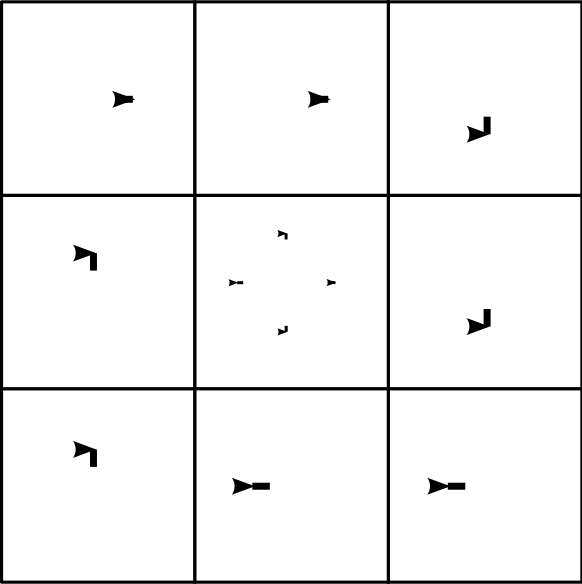
\includegraphics[width=0.8\columnwidth]{\visualspdf/frame/gridworld_around.pdf}
        \caption{W}
        \label{fig:gridwolrdgenericframesaround}
    \end{subfigure}
    \begin{subfigure}[b]{0.49\columnwidth}
        \centering
        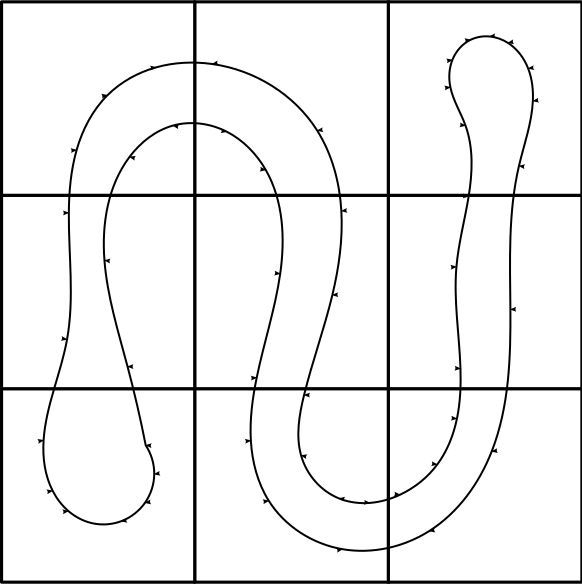
\includegraphics[width=0.8\columnwidth]{\visualspdf/frame/gridworld_loop.pdf}
        \caption{W}
        \label{fig:gridwolrdgenericframesloop}
    \end{subfigure}
\caption{Two examples of desired agent behavior that are harder to define in terms of rewards function.}
\label{fig:gridwolrdgenericframes}
\end{figure}

We note that it is always possible to represent the problems such that a fixed reward function allows to infer the policies of Figure~\ref{fig:gridwolrdgenericframesaround}~and~\ref{fig:gridwolrdgenericframesloop}. For Figure~\ref{fig:gridwolrdgenericframesaround} defining a reward function on the state-action space would be enough. For Figure~\ref{fig:gridwolrdgenericframesloop}, it is more challenging as the Markov properties are not respected, indeed it is necessary to known the previous position of the agent to predict its future position. Therefore the representation of the agent state should include the previous position of the agent, which increases the state space from 9 states to 81 states.

\subsubsection*{No need for planning skills}

\subsubsection*{Asynchronous instructions}

The interaction between our users and our robot would be easier if the robot could act continuously and the human would provide instruction when he deemed necessary. For example, in our pick and place scenario of chapter~\ref{chapter:lfui} it is boring for the user to provide feedback after each movement of the robot, it would be easier to wait the robot has displaced a cube to an other location. In addition, in some domains, the frequency of action is to high to afford waiting for a feedback signal between each action. Either the action would be so small that the user would not be able to judge the action, either the interaction flow would be dramatically affected by the many pauses in the task execution.

To allow for continuous operation of the robot, asynchronous delivery of signals should be accepted. A potential avenue is to consider a temporal function that distribute a signal event across some subset of previous robot events. This method has been used by Bradley Knox et al. in their TAMER framework \cite{knox2009interactively} using a data from a study of the distribution of human response times \cite{hockley1984analysis}.

\subsubsection*{Including social clues}

As for tackling the problem of asynchronous instructions, information known to be true for most interaction scenario can be included in the frame definition.  Such as whether the human is looking at the scene or not, but also the presence of other persons in the room, or that some objects are hiding parts of the world to the human eye, etc.



%%%%%%%%%%%%%%%%%%%%%%%%%%%%%%%%%%%%%%%%%%%%%%
%%%%%%%%%%%%%%%%%%%%%%%%%%%%%%%%%%%%%%%%%%%%%%
%%%%%%%%%%%%%%%%%%%%%%%%%%%%%%%%%%%%%%%%%%%%%%
%%%%%%%%%%%%%%%%%%%%%%%%%%%%%%%%%%%%%%%%%%%%%%
%%%%%%%%%%%%%%%%%%%%%%%%%%%%%%%%%%%%%%%%%%%%%%
\section{Future work in this domain}


\subsection{Technical challenges}

remove assumptions such as the one presented is limitation section

\subsection{Theoretical challenges}

We are not doing perfect science, all this is really empirical and lacks of clean mathematical work, such as proof and studies of the properties of the system. 

symmetry cases

By taking inspiration from the proof described in previous chapter, there is many fast imporvmenrt than can be done. Mainly by relaxinfg the assumtion that the user is perfect, or that each task is composed os half optimal and halfp non optimal state action pairs.


\subsection{Reaching tasks versus reward accumulation tasks}

difference between episodes based interaction and never ending 


\subsection{Applications}

This work opens a new perspective regarding the global challenge of interacting with machines. It has application to many interaction problems which requires a machine to learn how to interpret unknown communicative signals. A promising avenue, outside the BCI field, lies in human robot interaction scenarios where robots must learn from, and interact with, many different users who have their own limitations and preferences.

from the better, bci, assictive technologies

to the worth application, such as advertissing website, mouse movement on a website.

\subsection{Studying humans in the loop}
\label{chapter:limitations:userstudies}

\question{Do people want to have an open-ended choice about what signal to use? \\ Would they be more efficient?}

Only prerecorded datasets have been used. However, signals may change during the learning. For instance, people can try to adapt themselves to a robot if they believe the latter is not understanding properly. Or, brain signals are sensitive to the protocol, the duration of the experiment or even the percentage of errors made by the agent \cite{chavarriaga2010learning}. To which extend the behavior of our agent changes the properties of the teaching signal? 

Moreover, in real-world applications, users are usually told how to interact with machines. And having a free choice on some details of the interaction may finally become a disadvantage and lower perfomances. Do people want to have an open-ended choice about what signal to use? Would they be more efficient? When is it better to use a calibration procedure?

As we argued in the introduction, the work we presented is a starting point towards forms of adaptive interaction with non-technical users, that we may call fluid interaction learning. While we studied in this thesis properties of learning algorithms that will be needed for such an endeavor, it remains to be shown how they can be integrated within a full real-world human-robot interaction scenario and architecture so that the usability and acceptability of such system can be evaluated. Thus, user studies in particular will be a crucial next step of this work. The improvements described in previous section may be needed to reach acceptable levels of usability.

An interesting direction would be to consider the same experimental setup as the one used in chapter~\ref{chapter:humanexperiment} which allow to seamlessly use a human or a machine on either of the side of the interaction. A natural extension is therefore to replace the human builder by an agent using our algorithm. But one could also study active teaching algorithm \cite{cakmak2012algorithmic}, by replacing the teacher side by an artificial agent.

This kind of experiment would allow to study the same setup with both humans and artificial agents and may open new perspective in both human-robot interaction and experimental semiotic studies. By controlling some aspects of the interaction, on either of the interaction side, one could for example study how the agent behavior affect the teaching behavior of the human. But also study how the teaching behavior of a human influence the understanding and performance of the learner, whether the learner is a human or a machine. 

algorithm assumption on human behavior

discuss how the setup can be used in HRI, but also semiotic stuff...

Users comply with the frame implemented. Same meaning, optimal strategies, timing...

Assumption: The properties of the signals do not change wrt. the behavior of the agent

In relation to targeting fluid interaction learning, we will consider in the future how more complex kinds of instructions can be included in our formalism. Indeed, the possible teaching models used spontaneously by people can be more complex than the simple meaning correspondences we assumed \cite{thomaz2008teachable,Cakmak2010optimality}. Also the turn taking scheme could be made more natural, as the robot could ask questions \cite{cakmak2012designing} and accept asynchronous instructions.

Indeed, our current system can be restrictive for the user as the number of interaction increases quickly with the complexity of the size of the task and meaning spaces. However, we have shown that the system is able to use known sources of information, which in real-world interaction could be leveraged to keep the sample complexity low.

users are not ready maybe, they want intuitive interface, not adaptive.

human exp with a computer at one side, or with some signal not dipslaye,d or with delayed, or with ranodm possition...

cite mohammed chetouanni

\subsection{Creating meanings and interaction frames}

\question{Who create the frame functions?}

all this is very high level

learning the meaning is the natural next step, where very few work jave tackled it

how to learn the interaction hypothesis and interaction frame is a big problem, refer to thomas thesis.

coupled with a system that creates the frame, not neccessarily the meaning but at least generate some human behaviors.


The transition from raw input to higher level meaning is however not much investigated in science. Here our agent or robot already have the ability to categorize state, make plans and select what is relevant from the environment.

